% Options for packages loaded elsewhere
\PassOptionsToPackage{unicode}{hyperref}
\PassOptionsToPackage{hyphens}{url}
%
\documentclass[
  10pt,
]{article}
\usepackage{lmodern}
\usepackage{amssymb,amsmath}
\usepackage{ifxetex,ifluatex}
\ifnum 0\ifxetex 1\fi\ifluatex 1\fi=0 % if pdftex
  \usepackage[T1]{fontenc}
  \usepackage[utf8]{inputenc}
  \usepackage{textcomp} % provide euro and other symbols
\else % if luatex or xetex
  \usepackage{unicode-math}
  \defaultfontfeatures{Scale=MatchLowercase}
  \defaultfontfeatures[\rmfamily]{Ligatures=TeX,Scale=1}
\fi
% Use upquote if available, for straight quotes in verbatim environments
\IfFileExists{upquote.sty}{\usepackage{upquote}}{}
\IfFileExists{microtype.sty}{% use microtype if available
  \usepackage[]{microtype}
  \UseMicrotypeSet[protrusion]{basicmath} % disable protrusion for tt fonts
}{}
\makeatletter
\@ifundefined{KOMAClassName}{% if non-KOMA class
  \IfFileExists{parskip.sty}{%
    \usepackage{parskip}
  }{% else
    \setlength{\parindent}{0pt}
    \setlength{\parskip}{6pt plus 2pt minus 1pt}}
}{% if KOMA class
  \KOMAoptions{parskip=half}}
\makeatother
\usepackage{xcolor}
\IfFileExists{xurl.sty}{\usepackage{xurl}}{} % add URL line breaks if available
\IfFileExists{bookmark.sty}{\usepackage{bookmark}}{\usepackage{hyperref}}
\hypersetup{
  pdftitle={Dossier de candidature au poste de Maître de Conférences},
  pdfauthor={Adrien Méli},
  hidelinks,
  pdfcreator={LaTeX via pandoc}}
\urlstyle{same} % disable monospaced font for URLs
\usepackage[margin=1in]{geometry}
\usepackage{longtable,booktabs}
% Correct order of tables after \paragraph or \subparagraph
\usepackage{etoolbox}
\makeatletter
\patchcmd\longtable{\par}{\if@noskipsec\mbox{}\fi\par}{}{}
\makeatother
% Allow footnotes in longtable head/foot
\IfFileExists{footnotehyper.sty}{\usepackage{footnotehyper}}{\usepackage{footnote}}
\makesavenoteenv{longtable}
\usepackage{graphicx}
\makeatletter
\def\maxwidth{\ifdim\Gin@nat@width>\linewidth\linewidth\else\Gin@nat@width\fi}
\def\maxheight{\ifdim\Gin@nat@height>\textheight\textheight\else\Gin@nat@height\fi}
\makeatother
% Scale images if necessary, so that they will not overflow the page
% margins by default, and it is still possible to overwrite the defaults
% using explicit options in \includegraphics[width, height, ...]{}
\setkeys{Gin}{width=\maxwidth,height=\maxheight,keepaspectratio}
% Set default figure placement to htbp
\makeatletter
\def\fps@figure{htbp}
\makeatother
\setlength{\emergencystretch}{3em} % prevent overfull lines
\providecommand{\tightlist}{%
  \setlength{\itemsep}{0pt}\setlength{\parskip}{0pt}}
\setcounter{secnumdepth}{5}
\usepackage{fontawesome}
\usepackage{amsmath}
\usepackage{tipa}
\usepackage{moodle}
\usepackage{hyperref}
\usepackage{booktabs}
\usepackage[utf8]{inputenc}
\usepackage[light,sfdefault]{roboto}
%\usepackage{fourier}
%\usepackage{montserrat}
%\usepackage[T1]{fontenc}
%\usepackage[french]{babel}

% -----------------------------------------------------------------
% Hyper Setup
% -----------------------------------------------------------------
\hypersetup{
    %bookmarks=true,         % show bookmarks bar?
    unicode=false,          % non-Latin characters in Acrobat�s bookmarks
    pdftoolbar=true,        % show Acrobat�s toolbar?
    pdfmenubar=true,        % show Acrobat�s menu?
    pdffitwindow=false,     % window fit to page when opened
    pdfstartview={FitH},    % fits the width of the page to the window
    %pdftitle={},    % title
    pdfauthor={Adrien Meli},     % author 
    pdfsubject={Phonological rules},   % subject of the document
    pdfcreator={Creator},   % creator of the document
    pdfproducer={Producer}, % producer of the document
    pdfkeywords={Second Language Acquisition, French, English, phonology}, % list of keywords
    pdfnewwindow=true,     % links in new window
    colorlinks=true,       % false: boxed links; true: colored links
    linkcolor=black,          % color of internal links
    citecolor=black,        % color of links to bibliography
    filecolor=magenta,      % color of file links
    urlcolor=blue,           % color of external links
    bookmarksopen=false,
    anchorcolor=black,
    bookmarksnumbered=true,
    pdfpagemode=UseOutlines,    %None/UseOutlines/UseThumbs/FullScreen
    linktocpage=true
}

% ********************Captions and Hyperreferencing / URL **********************

% Captions: This makes captions of figures use a boldfaced small font.

\usepackage[margin=10pt,font=small,labelfont=bf,labelsep=endash]{caption}

% -----------------------------------------------------------------
% TABLE OF CONTENTS
% -----------------------------------------------------------------
\usepackage[dotinlabels]{titletoc}
\titlecontents{section}[0em] % entries are pushed to the rtight
  {} % code to change the appearance
  {} % section number: increase distance to push to the left
  {\hspace*{3.3em}}
  {\titlerule*[1.9mm]{.}\contentspage}
% remove subsections from TOC
\setcounter{tocdepth}{1}

% multi-line curly brackets

\newenvironment{rightbracedtext}
 {$\kern-\nulldelimiterspace\left.\begin{tabular}{@{}l@{}}}
 {\end{tabular}\right\}$}

\newenvironment{leftbracedtext}{$\left\{\begin{tabular}{@{}l}}{\end{tabular}\right.$}

%----------------------------------------------------------------------------------------
%	MARGINS
%----------------------------------------------------------------------------------------

%\usepackage{geometry} % Required for adjusting page dimensions and margins
%
%\geometry{
%	paper=a4paper, % Change to letterpaper for US letter
%	top=3cm, % Top margin
%	bottom=3cm, % Bottom margin
%	left=2cm, % Left margin
%	right=3cm, % Right margin
%	headheight=14pt, % Header height
%	footskip=1.4cm, % Space from the bottom margin to the baseline of the footer
%	headsep=1.2cm, % Space from the top margin to the baseline of the header
%	%showframe, % Uncomment to show how the type block is set on the page
%}
\usepackage{booktabs}
\usepackage{longtable}
\usepackage{array}
\usepackage{multirow}
\usepackage{wrapfig}
\usepackage{float}
\usepackage{colortbl}
\usepackage{pdflscape}
\usepackage{tabu}
\usepackage{threeparttable}
\usepackage{threeparttablex}
\usepackage[normalem]{ulem}
\usepackage{makecell}
\usepackage{xcolor}
\newlength{\cslhangindent}
\setlength{\cslhangindent}{1.5em}
\newenvironment{cslreferences}%
  {\setlength{\parindent}{0pt}%
  \everypar{\setlength{\hangindent}{\cslhangindent}}\ignorespaces}%
  {\par}

\title{Dossier de candidature au poste de Maître de Conférences}
\author{Adrien Méli}
\date{10 April, 2020}

\begin{document}
\maketitle

{
\setcounter{tocdepth}{1}
\tableofcontents
}
\begin{center}\rule{0.5\linewidth}{0.5pt}\end{center}

\quad \faEnvira \quad \texttt{adrienmeli@gmail.com}

\quad \faPhone \quad \texttt{01.55.43.89.87.}

\quad \faEnvelope \quad 236, rue de Charenton 75012 Paris

\href{https://adrienmeli.github.io/cv/}{\quad \faGithub \quad Version Github}

\begin{center}\rule{0.5\linewidth}{0.5pt}\end{center}

\pagebreak

\hypertarget{synthuxe8se}{%
\section{Synthèse}\label{synthuxe8se}}

TZR agrégé d'anglais

Actuellement en poste à l'École Supérieure des Arts et Industries Graphiques (École Estienne)

\hypertarget{thuxe8se-de-linguistique-anglaise}{%
\subsection{Thèse de linguistique anglaise}\label{thuxe8se-de-linguistique-anglaise}}

\begin{table}[H]
\centering
\begin{tabular}{>{\bfseries\raggedright\arraybackslash}p{2.5cm}>{\raggedright\arraybackslash}p{14cm}}
\toprule
Titre & A longitudinal study of the oral properties of the French-English interlanguage.\\
Sous-titre & A quantitative approach of the acquisition of the /I/-/i:/ and /U/-/u:/ contrasts.\\

Directeur & Nicolas Ballier, Professeur des Universités à Paris Diderot.\\

 & Sophie Herment, Professeur des Universités à Aix-Marseille.\\

\multirow[t]{-2}{2.5cm}{\raggedright\arraybackslash Rapporteurs} & Noël N'Guyen, Professeur des Universités à Aix-Marseille.\\

 & Emmanuel Ferragne, Maître de Conférences à Paris Diderot.\\

\multirow[t]{-2}{2.5cm}{\raggedright\arraybackslash Examinateurs} & Richard  Wright, Professeur des Universités à l'université de Washington.\\

Financement & Aucun. Thèse effectuée en parallèle de charges d'enseignement dans le secondaire à temps plein.\\
\bottomrule
\end{tabular}
\end{table}

\hypertarget{agruxe9guxe9-danglais}{%
\subsection{Agrégé d'anglais}\label{agruxe9guxe9-danglais}}

Agrégation externe d'anglais option B obtenue en juillet 2009.
Rang : 84.

\hypertarget{thuxe8mes-de-recherche}{%
\subsection{Thèmes de Recherche}\label{thuxe8mes-de-recherche}}

\begin{itemize}
\tightlist
\item
  Acquisition phonologique et phonétique
\item
  Parole spontanée (natifs et apprenants)
\item
  Alignement automatique de corpus oraux
\item
  Analyse statistique
\item
  Extraction automatique des données
\item
  Optimisation des traitements formantiques
\item
  Apprentissage automatique supervisé
\end{itemize}

\hypertarget{publications}{%
\subsection{Publications}\label{publications}}

\textbf{1} chapitre de livre.

\textbf{2} articles dans des actes de conférences internationales.

\textbf{1} article dans une revue en ligne française.

\hypertarget{enseignements}{%
\subsection{Enseignements}\label{enseignements}}

\textbf{15 ans} dans l'Enseignement Secondaire (lycée général principalement).

\textbf{2 ans } en BTS et DNMADE en école d'arts appliqués (ENSAAMA et Ecole Estienne).

\textbf{2 ans } de lectorat au Royaume-Uni (Queens' College à Cambridge) et aux États-Unis (University of California, Berkeley).

\textbf{1 semestre} de TD à l'université.

\textbf{1 séminaire} de douze heures à l'université.

\pagebreak

\hypertarget{curriculum-vitae}{%
\section{Curriculum Vitae}\label{curriculum-vitae}}

\hypertarget{formations-dipluxf4mes-et-concours}{%
\subsection{Formations, diplômes et concours}\label{formations-dipluxf4mes-et-concours}}

\begin{table}[H]
\centering
\begin{tabular}{>{\bfseries\raggedright\arraybackslash}p{2.5cm}>{\raggedright\arraybackslash}p{14cm}}
\toprule
2019 : & Qualifié aux sections 7 et 11 du Conseil National des Universités\\
2018 : & Doctorat de linguistique anglaise à l'université de Paris-Diderot.\\

2010 : & Master 2 Recherche de Linguistique Anglaise à Paris Diderot.\\

2009 : & Agrégation externe d'anglais (84ème).\\

2008 : & Concours d'Accès à l'Echelle de Rémunération des Professeurs Certifiés d'anglais (4ème).\\

 & Maîtrise d'anglais  à Paris-Nanterre.\\

\multirow[t]{-2}{2.5cm}{\raggedright\arraybackslash 1997-1998 :} & 2ème année de chinois à l’Institut National des Langues et Civilisations Orientales.\\

 & Licence d'anglais à Paris Nanterre.\\

\multirow[t]{-2}{2.5cm}{\raggedright\arraybackslash 1996-1997 :} & 1ère année de chinois à l’INALCO.\\

1993-1995 : & hypokhâgne et khâgne B/L à Stanislas (Paris 75006).\\

1993 : & Baccalauréat C (mention Assez Bien).\\
\bottomrule
\end{tabular}
\end{table}

\hypertarget{compuxe9tences-informatiques}{%
\subsection{Compétences informatiques}\label{compuxe9tences-informatiques}}

\begin{itemize}
\item
  \textbf{Systèmes :} Unix/Linux (Arch, Debian, Ubuntu)
\item
  \textbf{Maths :} \(R\)
\item
  \textbf{Aligneurs automatiques :} \href{http://www.sppas.org/}{sppas}, \href{https://arc.vt.edu/userguide/p2fa/}{p2fa}
\item
  \textbf{Languages :} \texttt{bash}, \href{http://www.fon.hum.uva.nl/praat/}{praat}, \texttt{Rmarkdown}, \LaTeX
\end{itemize}

\begin{quote}
À noter peut-être que j'utilise \href{https://www.vim.org}{Vim} pour gérer tous ces langages à la fois : adepte de la ligne de commande,
je suis convaincu que les interfaces graphiques me limitent en efficacité et productivité (mais c'est personnel !).

Ainsi créè-je tous mes documents (cours et questionnaires Moodle notamment), et exécutè-je tous mes scripts (Praat, R, bash), sous Vim, à l'aide de fonctions que j'ai moi-même écrites.

Bien qu'extérieure \emph{stricto sensu} aux activités de recherche et d'enseignement, cette façon de travailler les unifie toutefois, et le temps que j'ai consacré à la développer,
le plaisir qu'elle me procure, et enfin mon désir de la partager, m'imposaient d'en parler ici.
\end{quote}

\pagebreak

\hypertarget{expuxe9rience-denseignement}{%
\subsection{Expérience d'enseignement}\label{expuxe9rience-denseignement}}

\hypertarget{descriptif}{%
\subsubsection{Descriptif}\label{descriptif}}

L'essentiel de ma carrière s'est déroulée à enseigner l'anglais dans le secondaire, majoritairement
dans des lycées généraux de profils très différents.

Mes enseignements dans le Supérieur ont consisté à enseigner la phonologie anglaise en L2
pendant un semestre à raison de deux heures par semaine d'une part, et les fondamentaux du
logiciel de statistiques \(R\) à des masterants et doctorants lors d'un séminaire de 12 heures d'autre
part. J'ai aussi assumé des cours de grammaire et de traduction en Sciences de l'Éducation de 2004 à 2006, un semestre en classes préparatoires commerciales en 2008, puis 3 TD à l'\href{https://www.ipag.edu/en}{IPAG} au premier semestre de cette année.

À ceci s'ajoutent deux années à l'étranger où j'ai enseigné en tant que lecteur le français langue
étrangère : à six étudiants de Queens' College à Cambridge la première année (pour six heures
par semaine), puis à quatre groupe d'environ 25 étudiants à l'université de Californie à Berkeley la
deuxième année (pour une dizaine d'heures par semaine).

Enfin, j'ai enseigné l'anglais deux ans (cette année comprise) à des étudiants de BTS et de DNMADE à l'\href{http://www.ensaama.net/}{ENSAAMA} et l'\href{www.ecole-estienne.paris}{École Estienne}. Leurs besoins spécifiques de futurs imprimeurs, opérateurs pré-presse, graveurs, relieurs, designers de mode, ou encore typographes et illustrateurs furent une source réjouissante d'enrichissement pédagogique et lexical.

À l'exception de mes deux années de lectorat à Cambridge et Berkeley, tout mon travail universitaire depuis 2003, que ce soit les préparations au CAER-PC ou à l'Agrégation externe, ou encore
et bien sûr mon Mastère 2 et la rédaction de ma thèse de Doctorat, a été mené de front avec ma
fonction d'enseignant, que j'ai toujours exercée à temps plein en raison de nécessités financières.

\hypertarget{tableau-ruxe9capitulatif}{%
\subsubsection{Tableau récapitulatif}\label{tableau-ruxe9capitulatif}}

\begin{table}[H]
\centering\begingroup\fontsize{10}{12}\selectfont

\begin{tabular}{>{\bfseries\raggedright\arraybackslash}p{2.5cm}>{\raggedright\arraybackslash}p{14cm}}
\toprule
2019-2020 : & professeur d'anglais à l'École Estienne (Paris 75013)\\
2019-2020 : & Business English (3TD) à l'IPAG (Paris 75006)\\

 & professeur d’angais au lycée Gabriel FAURÉ (Paris 75013)\\

 & préparation à l’épreuve d’anglais du Concours Science Po Paris à Gabriel Fauré (2018)\\

 & professeur principal en Terminale ES (2018)\\

\multirow[t]{-4}{2.5cm}{\raggedright\arraybackslash 2014-2019 :} & professeur principal en Terminale L (2017)\\

2016 : & séminaire d'introduction aux statistiques et à \$R\$ à Paris Diderot\\

 & professeur d’anglais à l’École Nationale Supérieure des Arts Appliqués et des Métiers d’Art (ENSAAMA)\\

\multirow[t]{-2}{2.5cm}{\raggedright\arraybackslash 2013-2014 :} & professeur d’anglais à au collège Buffon (Paris 75015)\\

2012-2013 : & professeur d’anglais au lycée Carnot (Paris 75017)\\

2012 : & chargé de TD pour un cours d’oral et de phonologie anglaise à des étudiants de L2 à l’université Paris Diderot.\\

2011-2012 : & lecteur à l’université de Berkeley, Californie.\\

2010-2011 : & lecteur à Queens’ College, Cambridge (Royaume-Uni)\\

 & professeur d’anglais au lycée Georges Brassens (Paris 75019)\\

\multirow[t]{-2}{2.5cm}{\raggedright\arraybackslash 2009-2010 :} & professeur d’anglais au collège Edgar Varèse (Paris 75019)\\

 & professeur d’anglais à Sainte-Croix-de-Neuilly (Neuilly 92200)\\

 & niveaux : collège, lycée et classes préparatoires commerciales en 2008\\

 & créateur d’un échange de Troisièmes avec l’école The Perse à Cambridge (Royaume-Uni)\\

\multirow[t]{-4}{2.5cm}{\raggedright\arraybackslash 2001-2009 :} & professeur principal en Première pendant deux ans.\\

2004-2006 : & chargé de TD (grammaire et traduction) en L3 de Sciences de l’Éducation à l’université de Paris-Villetaneuse\\

1998-2000 : & professeur d’anglais remplaçant aux collèges et lycées des Oiseaux (Paris 75016)\\
\bottomrule
\end{tabular}
\endgroup{}
\end{table}

\pagebreak

\hypertarget{travaux-de-recherche}{%
\section{Travaux de recherche}\label{travaux-de-recherche}}

\hypertarget{publications-1}{%
\subsection{Publications}\label{publications-1}}

\begin{itemize}
\item
  Méli, A. \& Ballier, N. (2019). ``Analyse de la production de voyelles anglaises par des apprenants francophones, l'acquisition du contraste /I/--/i:/ à la lumière des k-NN'', \emph{Anglophonia}. Link: \href{https://journals.openedition.org/anglophonia/2109}{journals.openedition.org/anglophonia}
\item
  Méli, A. \& Ballier, N. (2015). Assessing L2 phonemic acquisition: a normalization-independent method? In \emph{Proceedings of the 18th International Congress of Phonetic Sciences}. (pp.~805-810) Glasgow, August 10 - 14 2015. Link: \href{https://www.internationalphoneticassociation.org/icphs-proceedings/ICPhS2015/Papers/ICPHS0805.pdf}{ipa.org}
\item
  Ballier, N. \& Méli, A. (2015). CV-patterned transfers among French speakers of English. In \emph{Proceedings of EPIP4, 4th International Conference on English Pronunciation: Issues \& Practices}. (pp.
  14--17) Prague, May 21 - 23, 2015. Link: \href{https://fu.ff.cuni.cz/epip4/docs/EPIP4-Proceedings.pdf}{cuni.cz}
\item
  Méli, A. (2013). ``Phonological acquisition in the French-English interlanguage: rising above the phoneme.'' In \emph{Automatic Treatment and Analysis of Learner Corpus Data}, edited by A. Ballier N. \& Díaz-Negrillo and P. Thompson, 207--26. Amsterdam: John Benjamins. Link: \href{https://benjamins.com/catalog/scl.59.13mel}{benjamins.com}
\end{itemize}

\hypertarget{communications}{%
\subsection{Communications}\label{communications}}

\begin{itemize}
\item
  Ballier, N. \& Méli, A. (2017) \emph{Analysing the emergence of vowel categorisation in a longitudinal learner
  corpus: the kernel estimate method}. EPIP2017, Caen, 17 mai 2015.
\item
  Méli, A. \& Ballier, N. (2016) \emph{Challenging the lexical set approach with classifiers for the investigation of the interphonology of /i/ vs.~/I/}. PAC2016, Aix-en-Provence, 29 septembre 2016.
\item
  Ballier, N. \& Méli, A. (2015) \emph{Learner phonetic variability and the lexicon: a pilot study for two phonemic contrasts}. Third Learner Corpus Research Conference, Radboud University, Cuijk / Nijmegen, Pays-Bas, 11 septembre 2015.
\item
  Méli, A. \& Ballier, N. (2015) \emph{Assessing L2 phonemic acquisition - RaDicHull: a normalization-independent method?} 18th International Congress of Phonetic Sciences, Glasgow, 10 août 2015.
\item
  Méli, A. (2015) \emph{Assessing phonemic acquisition - Phone-gating: a normalization-dependent procedure?} Workshop on Phonetic Learner Corpora Satellite workshop of ICPhS, Glasgow, 12 août 2015.
\item
  Ballier, N. \& Méli, A. (2015) \emph{CV-patterned transfers among French speakers of English}. 4th International Conference on English Pronunciation: Issues \& Practices, Prague, République tchèque, 21 mai 2015.
\item
  Méli, A. (2015) \emph{Vowel acquisition in the French-English interphonology}, Phonologie de l'Anglais Contemporain, Toulouse, 13 avril 2015.
\item
  Méli, A. \& Ballier, N. (2014) \emph{Investigating interlanguage stages: Vowel phonemic distinctions among French speakers of English}. 47th Annual Meeting of the Societas Linguistica Europaea, Adam Mickiewicz University, Pozna´n, Pologne, 11 septembre 2014.
\item
  Ballier, N. Méli, A. (2010) \emph{Designing an EFL learner corpus to analyse phonetic and phonological variation}. ICAME 2010, 26 mai 2010
\end{itemize}

\pagebreak

\hypertarget{axes-de-recherche}{%
\section{Axes de recherche}\label{axes-de-recherche}}

\hypertarget{ruxe9sumuxe9-de-la-thuxe8se}{%
\subsection{Résumé de la thèse}\label{ruxe9sumuxe9-de-la-thuxe8se}}

Ma thèse entreprend d'évaluer l'évolution de l'acquisition phonologique par des étudiants français
des contrastes anglais /\textipa{I}/-/i\textipa{:}/ et /\textipa{U}/-/u\textipa{:}/.

Le corpus étudié provient d'enregistrements de conversations spontanées menées avec des étudiants natifs. 12 étudiants, 9 femmes et 3 hommes, ont été suivis lors de 4 sessions espacées
chacune d'un intervalle de six mois.

L'approche adoptée est résolument quantitative, et agnostique quant aux théories d'acquisition
d'une deuxième langue.

Afin d'estimer les éventuels changements de prononciation, une procédure d'alignement automatique et d'extraction des données acoustiques a été conçue à partir du logiciel PRAAT (Boersma and Weenink (\protect\hyperlink{ref-praat}{2019})). Dans un premier temps, deux autres logiciels (SPPAS et P2FA, Bigi (\protect\hyperlink{ref-sppas2012}{2012}) et Yuan and Liberman (\protect\hyperlink{ref-p2fa}{2008})) avaient aligné les transcriptions des enregistrements au phonème près. Plus de 90 000
voyelles ont ainsi été analysées. Les données extraites sont constituées d'informations telles que
le nombre de syllabes du mot, de sa transcription acoustique dans le dictionnaire, de la structure
syllabique, des phonèmes suivant et précédant la voyelle, de leur lieu et manière d'articulation, de
leur appartenance ou non au même mot, mais surtout des relevés formantiques de F0, F1, F2, F3
et F4. Ces relevés formantiques ont été effectués à chaque pourcentage de la durée de la voyelle
afin de pouvoir tenir compte des influences des environnements consonantiques sur ces formants.
Par ailleurs, des théories telles que le changement spectral inhérent aux voyelles (Nearey and Assmann (\protect\hyperlink{ref-nearey1986}{1986}), Morrison and Nearey (\protect\hyperlink{ref-morrison2006}{2006}), Hillenbrand (\protect\hyperlink{ref-hillenbrand2012}{2012}), Morrison (\protect\hyperlink{ref-morrison2012}{2012})), ou des méthodes
de modélisation du signal telles que la transformation cosinoïdale discrète (Harrington 2010) requièrent que soient relevées les valeurs formantiques des voyelles tout au long de leur durée.

Trois autres corpus se sont rajoutés à ce corpus principal et ont subi le même traitement :

\begin{enumerate}
\def\labelenumi{\arabic{enumi}.}
\item
  des enregistrements d'un texte en français lu par les mêmes étudiants (2 902 voyelles extraites);
\item
  une liste de mots anglais contenant toutes les voyelles de l'anglais, à raison de quatre mots
  par voyelle, aussi lue par ces étudiants (1 750 voyelles extraites);
\item
  un ensemble d'enregistrements de natifs en conversation spontanée réupérés à la radio
  (4 973 voyelles extraites).
\end{enumerate}

Sont successivement étudiées la fiabilité de l'extraction automatique, les distributions statistiques
des valeurs formantiques de chaque voyelle et les méthodes de normalisation appropriées aux
conversations spontanées. Les différences entre les locuteurs sont ensuite évaluées en analysant
tour à tour et après normalisation les changements spectraux, les valeurs formantiques à la moitié
de la durée de la voyelle et les transformations cosinoïdales. Ces évalutions sont complétées par
des comparaisons avec les résultats obtenus en analysant les données des trois autres corpus --
notamment en utilisant les données natives comme valeurs de référence.

Les méthodes déployées sont les \(k\) plus proches voisins, les analyses discriminantes quadratiques
et linéaires, ainsi que les régressions linéaires à effets mixtes.

Une conclusion temporaire de ce travail est que l'acquisition du contraste /I/-/i:/ semble plus
robuste que celle de /U/-/u:/, ce qui invite à prendre en compte d'autres paramètres que le niveau
segmental, tels que structure syllabique, nature grammaticale ou fréquence d'occurrence, lors de l'évaluation d'une acquisition de contraste phonémique.

\pagebreak

\hypertarget{projets-de-recherche}{%
\subsection{Projets de recherche}\label{projets-de-recherche}}

Le projet qui recouperait mes compétences, mon activité et mon intérêt consisterait
à créer un outil de diagnostic automatique de prononciation
vocalique\footnote{L'\href{https://sites.uclouvain.be/elen/}{ICTEAM-ELEN} de l'université de
  Louvain travaille sur un outil similaire, l'application
  \href{https://www.speasy.app/}{speakeasy}. Je suis actuellement en contact avec les
  concepteurs, Zoé Broisson, Benoît Macq et Georgios Athansopoulos, pour une
  collaboration éventuelle.}.

La figure \ref{fig:diagno0} représente le fonctionnement d'un tel outil, les couleurs
symbolisant l'état d'avancement de chaque étape :

\begin{itemize}
\item
  en vert foncé, ce qui est prêt et opérationnel ( les procédures d'alignement et d'extraction des données).
\item
  en vert clair ce pour quoi les bases sont posées mais l'ensemble doit être étoffé (le corpus natif, les méthodes de classification).
\item
  en rouge clair ce qui demeure problématique sur le plan théorique (traitement formantique) ou pratique (formulation des recommandations).
\item
  en rouge foncé, ce qui reste à faire (déploiement sur une plate-forme).
\end{itemize}

\begin{figure}
 
 {\centering 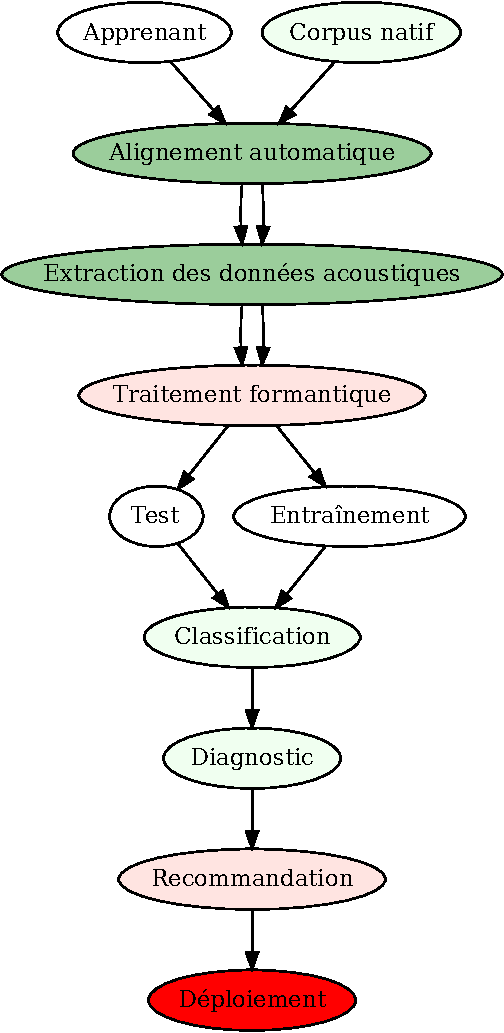
\includegraphics[width=468px,height=0.5\textheight]{index_files/figure-latex/diagno0-1} 
 
 }
 
 \caption{Processus de diagnostic automatique}\label{fig:diagno0}
 \end{figure}

Le principe est le suivant : l'enregistrement (lu ou spontané) d'un apprenant est transcrit et annoté selon les mêmes procédures qu'un corpus natif pré-existant.
Les valeurs formantiques de chaque voyelle de l'apprenant sont comparées à celles des natifs de même sexe \textbf{dans les mêmes mots et les mêmes syllabes}.

Ces valeurs sont ensuite classées selon une méthode d'apprentissage supervisé de type \(k\)-NN, les valeurs natives constituant l'ensemble d'entraînement, celles de l'apprenant, l'ensemble de test\footnote{Plus d'explications sont disponibles dans l'article publié dans \protect\hyperlink{anglophonia}{Anglophonia} et soumis en cas d'audition.}.

La qualité de la classification, ainsi que la nature des écarts éventuels avec les valeurs natives, permettent d'établir un état des lieux de la qualité de prononciation. De cet état des lieux peuvent être formulées des recommandations claires et précises (par exemple, ``arrondir davantage les lèvres'' plutôt que ``la F2 est trop haute''). L'ensemble du processus, de l'enregistrement à la formulation des recommandations, pourrait être déployé sur une plate-forme de type Moodle.

L'un des enjeux cruciaux consiste à déterminer :

\begin{enumerate}
\def\labelenumi{\arabic{enumi}.}
\tightlist
\item
  la manière de traiter les formants (faut-il les normaliser ? À quel endroit de la durée de la voyelle faut-il prendre leur valeur ? Faut-il prendre la F3 ? La F4 ? Modéliser les courbes formantiques sur toute la durée ?)
\item
  quel méthode de classification utiliser (\(k\)-NN, machine à vecteurs de support, réseau de neurones artificiels, etc.).
\end{enumerate}

Toutes ces procédures devraient idéalement être comparées (en espérant une convergence de résultats\ldots) et évaluées (en fonction notamment de leur fiabilité et de leur poids computationnel).

À noter enfin que l'outil pourrait être élargi (par ordre croissant de complexité) :

\begin{itemize}
\item
  à la prononciation des consonnes (l'alignement automatique étant effectué au niveau segmental).
\item
  à l'intonation (j'ai étendu récemment ma méthode à MOMEL et INTSINT\footnote{\emph{C.f.} Hirst and Espesser (\protect\hyperlink{ref-hirst1993}{1993})} après avoir obtenu la charge d'aligner les enregistrements du \href{http://www.transfers.ens.fr/eiida-etudes-interdisciplinaires-et-interlinguistiques-du-discours-academique}{corpus EIIDA}).
\item
  à la complexité syntaxique (je suis en contact avec Thomas Gaillat (Rennes 2)
  pour l'exploration des métriques de l'écrit et l'oral et l'intégration dans Moodle de visualisation de performances).
\end{itemize}

\hypertarget{responsabilituxe9s-administratives}{%
\section{Responsabilités administratives}\label{responsabilituxe9s-administratives}}

J'ai été responsable pendant quatre ans d'un échange scolaire en classe de Troisième que j'ai créé avec une école anglaise, The Perse, à Cambridge.

La responsabilité administrative essentielle que j'ai assumée depuis lors est celle de
professeur principal en Terminale de 2017 à 2019, où j'ai dû
notamment aider les élèves à bâtir leurs projets d'orientation dans le
respect des nouvelles contraintes de PARCOURSUP.

\hypertarget{anglophonia}{%
\section{Documents soumis en cas d'audition}\label{anglophonia}}

\begin{itemize}
\item
  Méli, A. \& Ballier, N. (2019). ``Analyse de la production de voyelles anglaises par des apprenants francophones, l'acquisition du contraste /I/--/i:/ à la lumière des k-NN'', \emph{Anglophonia}. Link: \href{https://journals.openedition.org/anglophonia/2109}{journals.openedition.org/anglophonia}
\item
  Méli, A. \& Ballier, N. (2015). Assessing L2 phonemic acquisition: a normalization-independent method? In \emph{Proceedings of the 18th International Congress of Phonetic Sciences}. (pp.~805-810) Glasgow, August 10 - 14 2015. Link: \href{https://www.internationalphoneticassociation.org/icphs-proceedings/ICPhS2015/Papers/ICPHS0805.pdf}{ipa.org}
\item
  Méli, A. (2013). ``Phonological acquisition in the French-English interlanguage: rising above the phoneme.'' In \emph{Automatic Treatment and Analysis of Learner Corpus Data}, edited by A. Ballier N. \& Díaz-Negrillo and P. Thompson, 207--26. Amsterdam: John Benjamins. Link: \href{https://benjamins.com/catalog/scl.59.13mel}{benjamins.com}
\end{itemize}

\hypertarget{ruxe9fuxe9rences-bibliographiques}{%
\section*{Références bibliographiques}\label{ruxe9fuxe9rences-bibliographiques}}
\addcontentsline{toc}{section}{Références bibliographiques}

\hypertarget{refs}{}
\begin{cslreferences}
\leavevmode\hypertarget{ref-sppas2012}{}%
Bigi, B. 2012. ``SPPAS: a tool for the phonetic segmentations of Speech.'' Istanbul.

\leavevmode\hypertarget{ref-praat}{}%
Boersma, Paul, and David Weenink. 2019. ``Praat: Doing Phonetics by Computer {[}Computer Program{]}. Version 6.1.07, Retrieved 26 November 2019 from Http://Www.praat.org/.'' 2019.

\leavevmode\hypertarget{ref-hillenbrand2012}{}%
Hillenbrand, James M. 2012. ``Static and Dynamic Approaches to Vowel Perception.'' In \emph{Vowel Inherent Spectral Change}, 9--30. Springer Science \(+\) Business Media. \url{https://doi.org/10.1007/978-3-642-14209-3_2}.

\leavevmode\hypertarget{ref-hirst1993}{}%
Hirst, Daniel, and Robert Espesser. 1993. ``Automatic Modelling of Fundamental Frequency Using a Quadratic Spline Function.'' \emph{Travaux de L'Institut de Phonétique d'Aix} 15: 75--85.

\leavevmode\hypertarget{ref-morrison2012}{}%
Morrison, Geoffrey Stewart. 2012. ``Theories of Vowel Inherent Spectral Change.'' In \emph{Vowel Inherent Spectral Change}, 31--47. Springer Science \(+\) Business Media. \url{https://doi.org/10.1007/978-3-642-14209-3_3}.

\leavevmode\hypertarget{ref-morrison2006}{}%
Morrison, G. S., and T. M. Nearey. 2006. ``A Cross-Language Vowel Normalisation Procedure.'' \emph{Canadian Acoustics} 34 (3): 94--95.

\leavevmode\hypertarget{ref-nearey1986}{}%
Nearey, T., and P. F. Assmann. 1986. ``Modeling the Role of Vowel Inherent Spectral Change in Vowel Identification.'' \emph{Journal of the Acoustical Society of America} 125: 2387.

\leavevmode\hypertarget{ref-p2fa}{}%
Yuan, J., and M. Liberman. 2008. ``Speaker Identification on the SCOTUS Corpus.'' \emph{Journal of the Acoustical Society of America,} 123(5): 5687.
\end{cslreferences}

\end{document}
